\subsection{Empirical Analysis of WSM Schedule}
In this section, we conduct a comprehensive empirical study to dissect the WSM schedule. We aim to understand the key factors influencing its performance, its robustness across different training scenarios, its interaction with conventional decay mechanisms, and its broader implications on model dynamics.

\subsubsection{Robustness Across Pre-training Process}
Beyond applying WSM as a final step on a high-quality dataset, we also evaluated its utility and robustness throughout the entire pre-training lifecycle. To achieve this, we conducted a comparative analysis at various intermediate stages of a long training run, comparing the performance of a model produced by our computationally-frugal WSM merging against one produced by initiating a full, resource-intensive learning rate (LR) decay.
As shown in Figure \ref{fig:weight_a}, although the performance gains over WSD are not as significant as when switching to high-quality data, we find that the performance of models generated via WSM merging consistently and closely mirrors the results of a true LR anneal. In the figure, the gray line represents the base model trained with a constant LR. The blue lines show the performance of WSM models, which were created by mean-merging four checkpoints from within the preceding 100B-token merge duration. The red lines represent full 100B-token decay runs initiated at the 2T, 4T, 6T, 8T, and 10T token milestones. This result establishes WSM as a reliable, high-fidelity proxy for estimating a model's post-anneal potential at any point during training. Consequently, it can provide effective assessment throughout the pre-training phase, eliminating the need to launch multiple, expensive decay runs to gauge the model's true strength.


\subsubsection{Impact of Merging Algorithm}
As derived in Section~\ref{Theoretical}, the checkpoint merging process can be viewed as an approximation of a LR decay schedule, where the weighting scheme of the merge is analogous to the functional form of the decay curve. For instance, a simple mean average is analogous to a linear decay curve. An Exponential Moving Average (EMA) would correspond to a convex exponential decay curve.
Existing works~\citep{1sqrt} and our prior experiments with the WSD schedule revealed a performance hierarchy among decay curves: concave schedules (e.g., inverse square root) and linear schedules outperform convex schedules (details are provided in Appendix~\ref{app:add_exp}). Building on these findings, we hypothesize that a merging algorithm designed to approximate decay curves that have been proven effective in WSD scheduling will similarly yield better results.


Based on Theorem~\ref{thm:inverse}, we experimentally compare three merging algorithms: one using our theorem-generated weights to approximate 1-\textit{sqrt} decay, another using simple mean averaging, and a third using EMA.
Our experimental results in Table~\ref{tab:merge_comparison_fixed} validate this hypothesis. While the merge method outperforms decay, the 1-\textit{sqrt} merge approach shows slight advantages over Mean, and both are markedly better than EMA. This finding reinforces the theoretical connection between checkpoint merging and LR decay, suggesting that the benefits of superior decay schedules can be effectively captured through carefully designed merging weights.



\subsubsection{Impact of Merging Duration and Granularity}
\begin{figure*}[t]
    \centering
    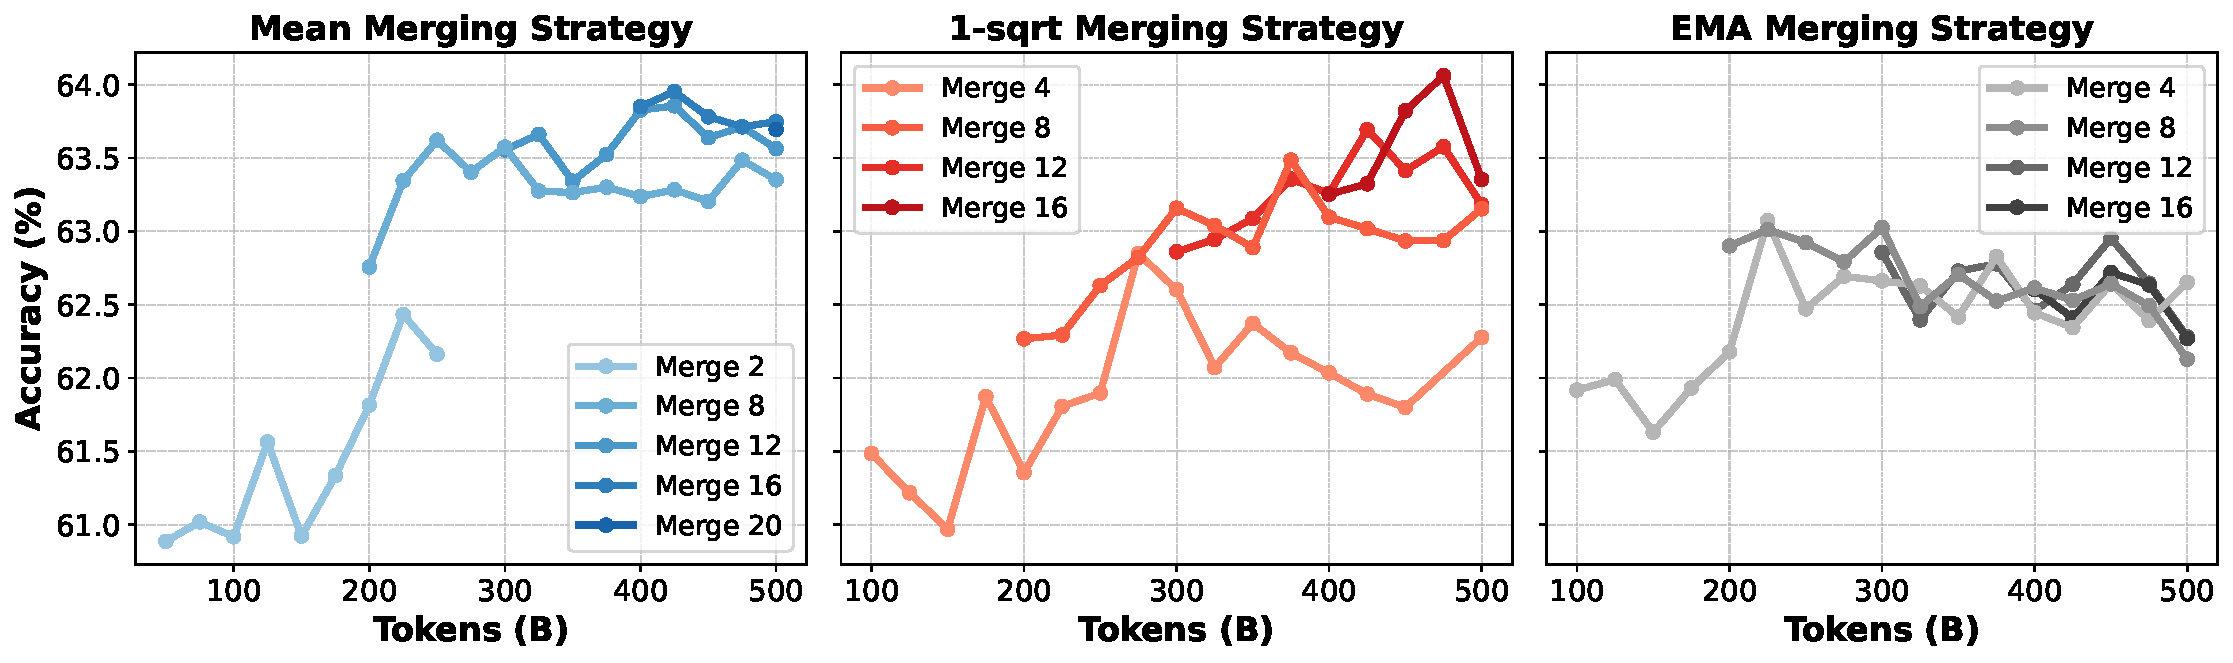
\includegraphics[width=1\textwidth]{figs/window.pdf}
    \caption{\textbf{Merge duration analysis across algorithms.}``Merge 4'' indicates merging the most recent 4 checkpoints, with each checkpoint saved at 25B-token intervals.}
    \label{fig:window}
\end{figure*}

We further investigate in detail the impact of different merge durations (window sizes) on various algorithms.
First, different merge durations essentially correspond to decaying with varying amounts of data.
As shown in Figure \ref{fig:window}, when comparing the best-performing checkpoints across the entire merging trajectory for both mean and 1-\textit{sqrt} merging algorithms, larger merging windows tend to yield better results.
However, this advantage gradually diminishes as the window size increases. This observation aligns with previous practical LR decay experiments, where simply increasing the amount of annealing data shows diminishing returns and may eventually fail to provide further improvement. These findings further strengthen the connection between LR decay and checkpoint merging.
For EMA merging, its performance is significantly inferior to other algorithms and shows no clear variation with merge durations. This may indicate that EMA is not an effective merging algorithm (also suggesting that the convex nature may not represent an optimal decay curve).

Then we further investigate the granularity of checkpoint merging, i.e., the interval between saved checkpoints used for merging. Finer-grained merging represents a more precise approximation of the true decay curve. The results in Table~\ref{tab:Granularity} show that finer-grained merging tends to achieve better performance. However, frequent checkpoint saving imposes storage overhead, requiring careful trade-off considerations.

\begin{table}[htbp]
  \centering
  \small
  \caption{\textbf{Impact of merging algorithm.} }
  \label{tab:merge_comparison_fixed}
  \begin{tabularx}{\textwidth}{ c c C C C C C C }
    \toprule
    &  & General Knowledge & Language Modeling & Math & Code & Professional Knowledge & Overall Average\\
    \midrule
    \multirow{1}{*}{Decay}
    &  1-\textit{sqrt}     & 69.06 & 67.78 & 57.49 & 64.88& 53.46 & 62.67 \\
    \midrule
    \multirow{3}{*}{Merging}
    & EMA                 & 69.05 & 67.64 & 58.81 & 64.19 & 54.44 & 63.01 \\
    & Mean                & 70.22 & \textbf{68.67} & 58.81 & 65.58& \textbf{56.04} & 63.95 \\
    &  1-\textit{sqrt}       & \textbf{70.27} & 68.26 & \textbf{59.65} & \textbf{65.70} & 55.42 & \textbf{64.06} \\
    \bottomrule
  \end{tabularx}
\end{table}


\begin{table}[htbp]
  \centering
  \small
  \caption{\textbf{Comparison of different saving/merging intervals within an 80B-token merge duration.} For example, (5B,16) indicates that saving every 5B tokens while merging the latest 16 checkpoints.}
  \label{tab:Granularity}
  \begin{tabularx}{\textwidth}{ C c C C C C C C }
    \toprule
    Merging Granularity & & General Knowledge & Language Modeling & Math & Code & Professional Knowledge & Overall Average\\
    \midrule
    (5B,16)                 & & \textbf{69.46} & 79.95 & 57.07 & \textbf{64.68} & 53.82 & 63.63 \\
    (10B,8)                & & 69.23 & 80.00 & \textbf{57.94} & 64.39& 53.78 & \textbf{63.78} \\
    (20B,4)                & & 69.29 & \textbf{80.29} & 56.79 & 63.87 & \textbf{54.19} & 63.36 \\
    (40B,2)                & & 68.47 & 79.83 & 56.57 & 63.59 & 52.20 & 62.77 \\
    (80B,1)                & & 67.47 & 64.98 & 55.07 & 61.69 & 51.61 & 60.33 \\
    \bottomrule
  \end{tabularx}
\end{table}

\subsubsection{On the Compatibility of Merge and Decay}
Given that checkpoint merging effectively simulates LR decay, a natural question arises: can merging and decay be combined to achieve synergistic performance gains? We investigate this by testing two hybrid approaches. (1) Decay-then-Merge: We first apply a standard decay schedule and then merge checkpoints selected from within the decay phase. (2) Merge-then-Decay: We further apply a decay schedule to the resulting merged model.
\begin{figure*}[t]
    \centering
    \begin{subfigure}[t]{0.32\textwidth}
        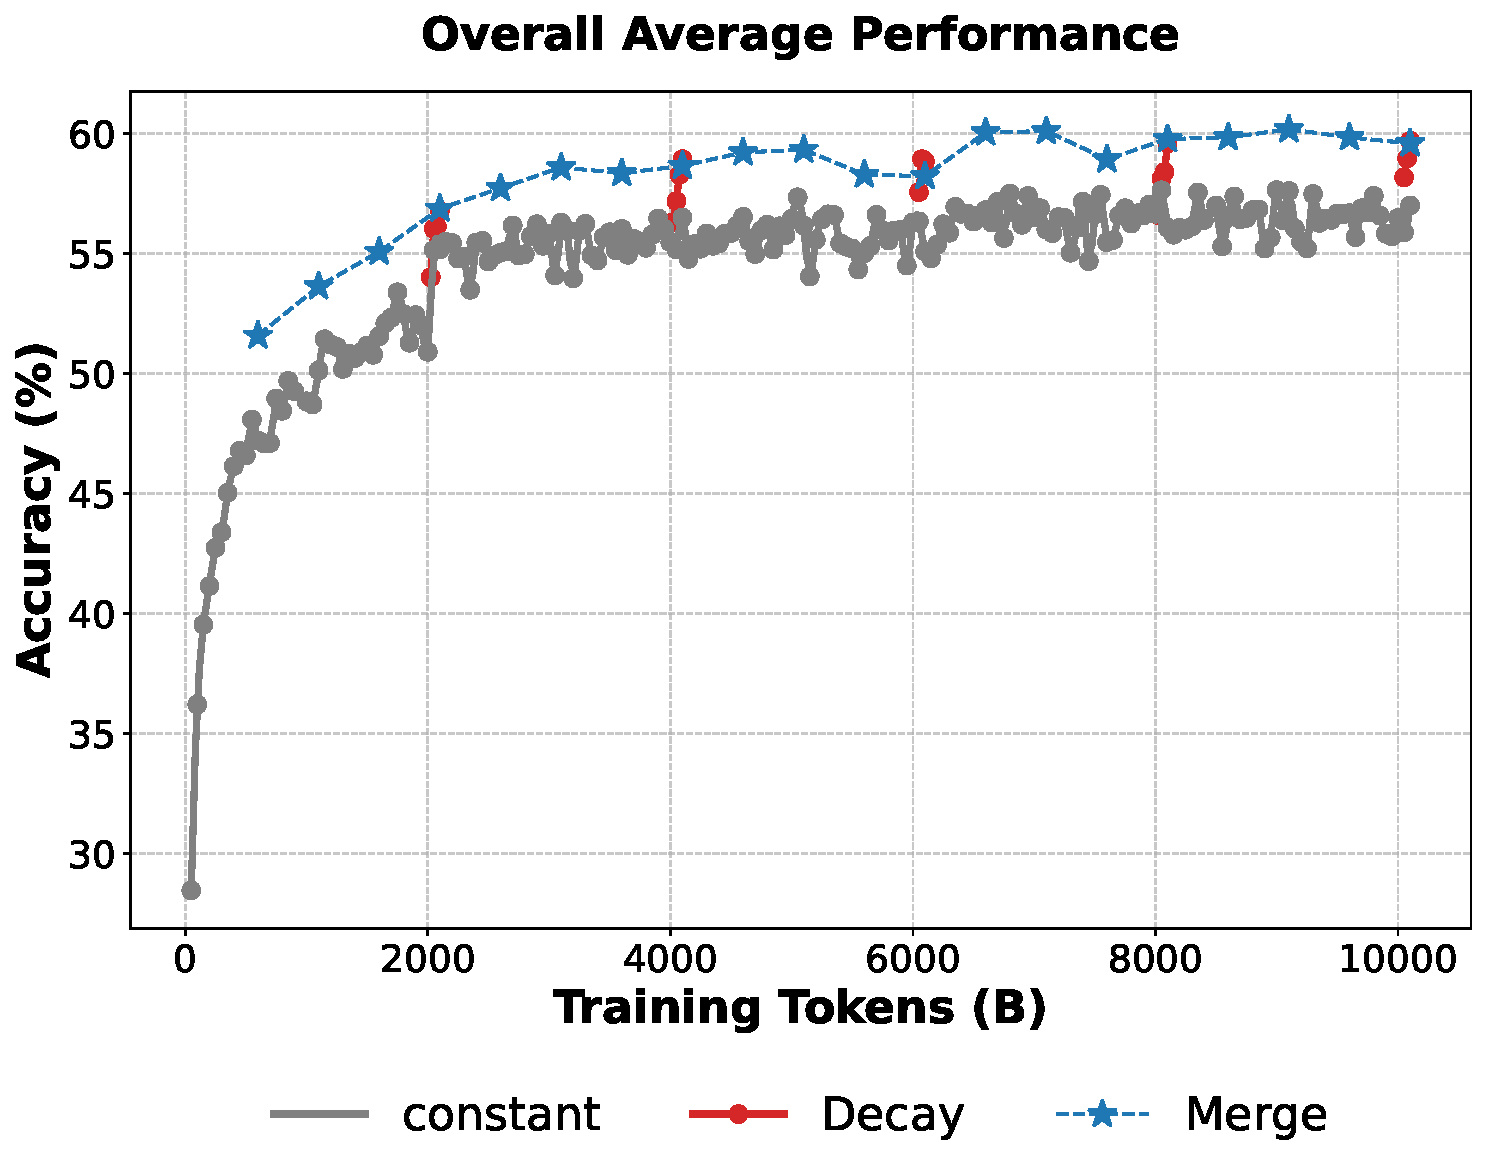
\includegraphics[width=\linewidth]{figs/constant.pdf}
        \caption{}
        \label{fig:weight_a}
    \end{subfigure}
    \hfill
    \begin{subfigure}[t]{0.32\textwidth}
        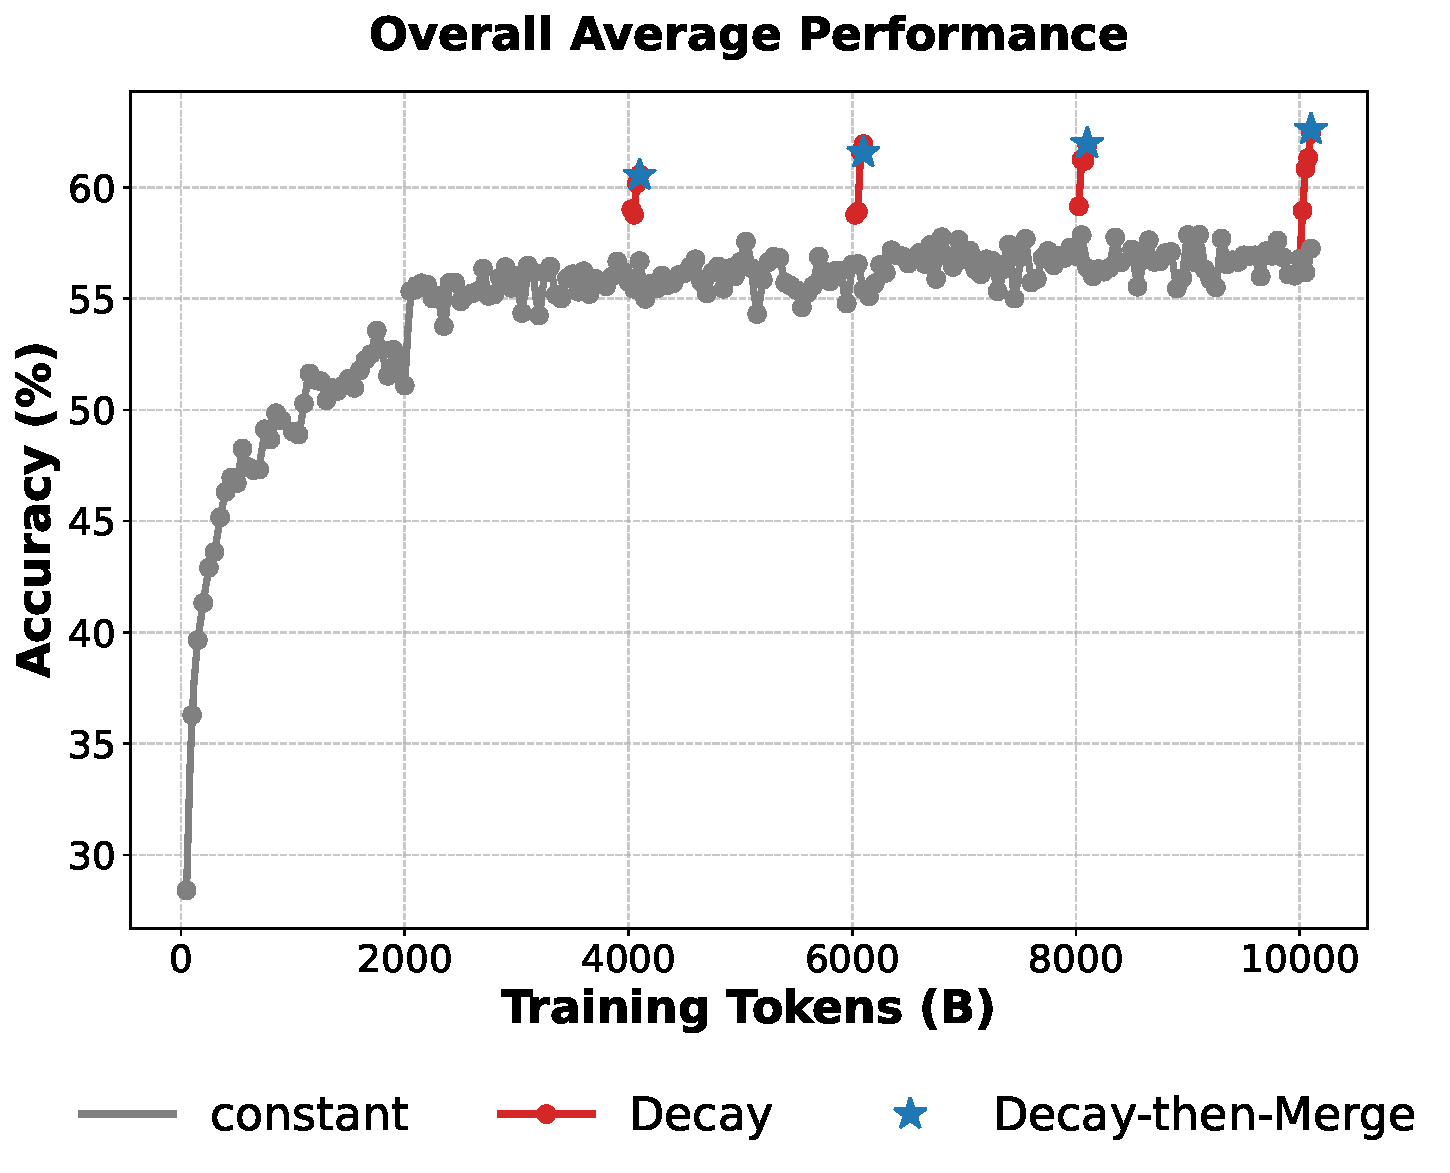
\includegraphics[width=\linewidth]{figs/decay_merge.pdf}
        \caption{}
        \label{fig:weight_b}
    \end{subfigure}
    \hfill
    \begin{subfigure}[t]{0.32\textwidth}
        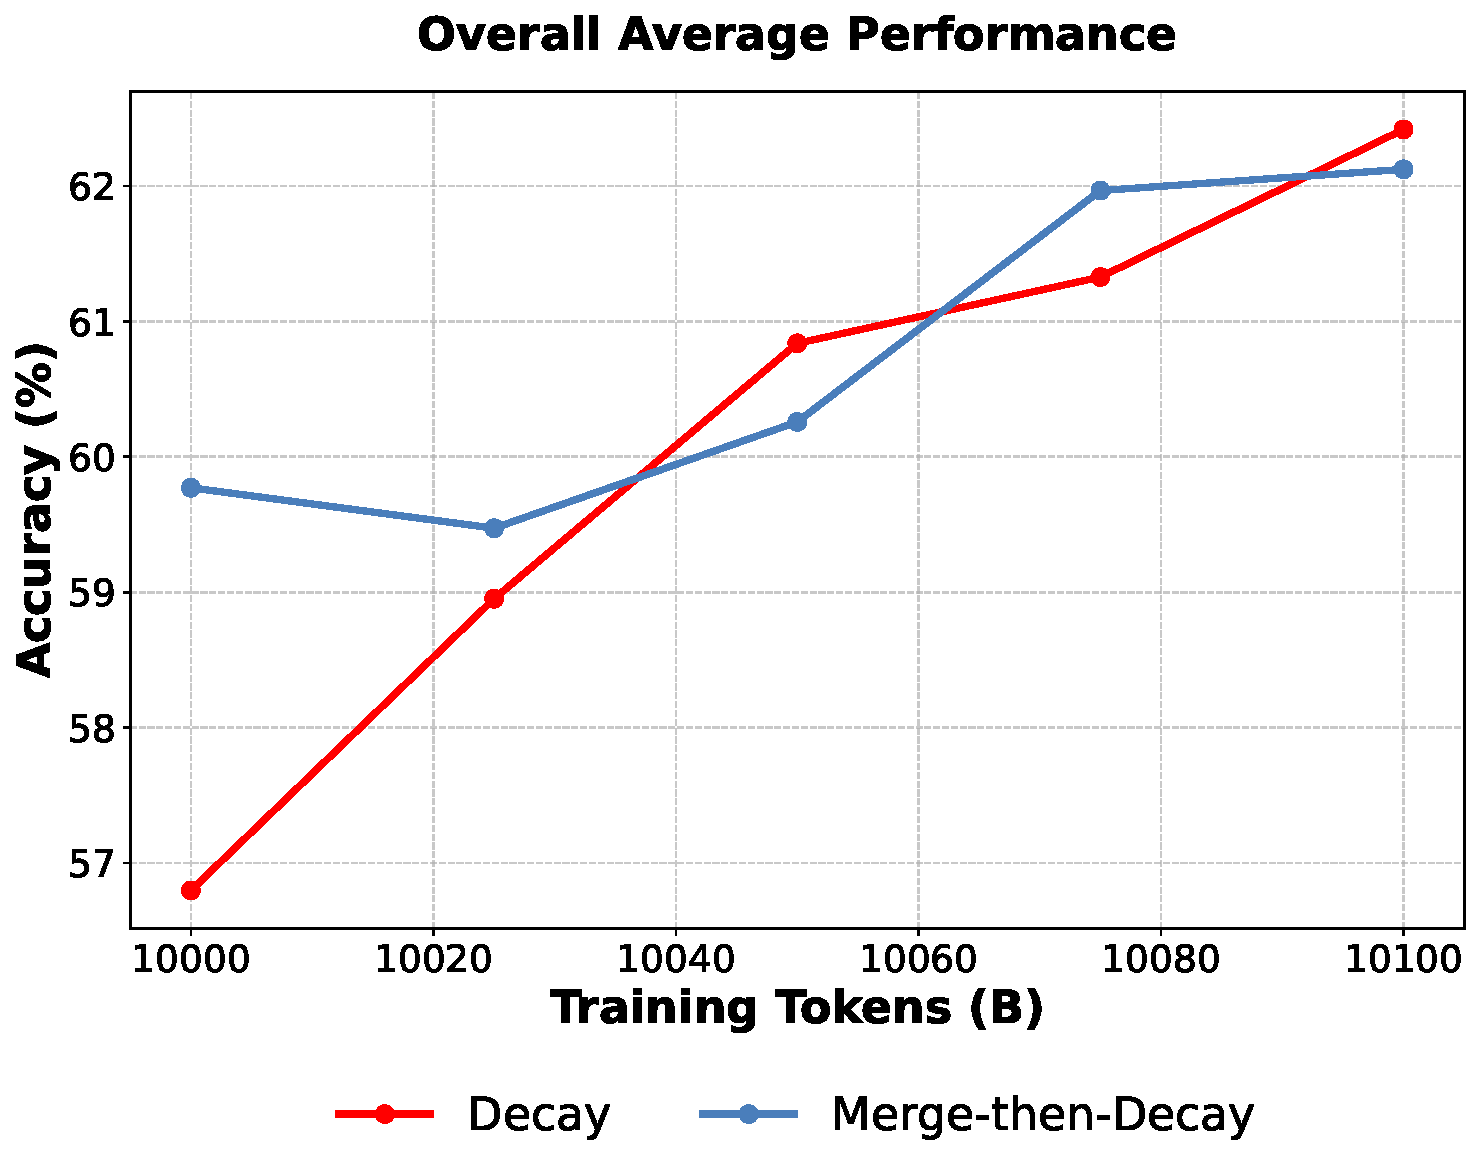
\includegraphics[width=\linewidth]{figs/merge_decay.pdf}
        \caption{}
        \label{fig:weight_c}
    \end{subfigure}
    \caption{(a) A comparison of checkpoint merging (WSM) and true LR decay (WSD) across a long pre-training run. (b) Investigating the effect of applying merging within a decay phase (Decay-then-Merge). (c) Investigating the effect of applying LR decay after checkpoint merging (Merge-then-Decay).}
    \label{fig:all}
\end{figure*}
As shown in Figures \ref{fig:weight_b} and \ref{fig:weight_c}, the hybrid approach failed to yield any improvement in either configuration, although the Merge-then-Decay model showed better performance at the beginning of its training. For the Decay-then-Merge experiment (Figure \ref{fig:weight_b}), the blue stars represent the results of merging checkpoints selected along the decay trajectories (red lines), which were initiated at various pre-training milestones (4T, 6T, 8T, 10T). For the Merge-then-Decay experiment (Figure \ref{fig:weight_c}), we compare a decay run initiated from a WSM model (blue line)—created by merging four checkpoints from the 9.8T to 10T token interval—against a standard decay baseline initiated from a single 10T checkpoint (red line). These results suggest that checkpoint merging and LR decay are not complementary but rather alternative pathways to a similar optimization objective.

\subsubsection{Impact on MoE Load Balancing}
\begin{table}[htbp]

\centering
\caption{\textbf{Impact on MoE load balancing.} The WSM strategy demonstrates improved expert utilization (lower load balancing violation scores) with a slightly higher language modeling loss.}
\begin{tabular}{lccc}
\toprule
 & language modeling loss & mean\_global\_max\_violation & mean\_global\_min\_violation \\
\midrule
WSD & 0.675 & 0.601 & 0.322 \\
WSM & 0.697 & \textbf{0.545} & \textbf{0.201} \\
\bottomrule
\end{tabular}
\label{route}
\end{table}

We provide a more in-depth analysis of the implications of WSM on MoE router balance in Table~\ref{route}. Specifically, the violation for a single expert is calculated as its relative deviation from the average load within its layer\footnote{For a single layer, let $L$ be the vector of token loads for its experts and $\mu = \text{mean}(L)$, $\text{max\_violation} = \frac{\lvert \max(L) - \mu \rvert}{\mu}$ and $\text{min\_violation} = \frac{\lvert \min(L) - \mu \rvert}{\mu}$}. The mean\_global\_max\_violation represents the average of the highest violations across all layers (measuring the severity of ``overloaded'' experts), while mean\_global\_min\_violation averages the violations for the least-utilized experts (measuring the risk of ``routing collapse'').
When comparing the merged checkpoint with a decayed checkpoint, the merged checkpoint achieves more balanced routing, although its loss is slightly higher.
We argue that this trade-off—a marginally higher loss for superior downstream performance—is indicative of enhanced generalization rather than overfitting to the training data.
More analysis of the parameter distribution is provided in Appendix \ref{parameter}. 


\subsection{Parameter Trajectories and Model Performance: Constant LR with Merge vs. LR Decay}
To visually analyze the correlation between model parameters and performance during training, we employ t-SNE~\citep{vanDerMaaten2008} dimensionality reduction to project the weight matrix of a specific layer into the 2-dimensional embedding space.
This projection is combined with performance evaluations to generate the composite contour map illustrated in Figure \ref{fig:wss_ling_mini_merge_ckpt_weight_distributions_for_paper}.
The directional arrows in the visualization explicitly illustrate the parameter trajectories across both constant and decay phases.
Our experimental analysis revealed two principal findings:
1) During the decay phase, model parameters gradually converge toward the merged model solution space, which achieves superior performance compared to checkpoints with a constant LR.
2) The LR reduction in the decay phase enables more precise parameter refinement than the expansive exploration observed under constant LR. This controlled convergence facilitates localization of nearby optimal solutions. 
We confirm the speculation of previous work~\cite{wen2024understanding}, 
and formalize this dynamic with an analogy: constant LR training resembles traversing a ``canyon'' with oscillating steps, while merging resembles finding a ``river'' at the canyon floor that guides efficient convergence. 

\begin{figure*}[t]
    \centering
    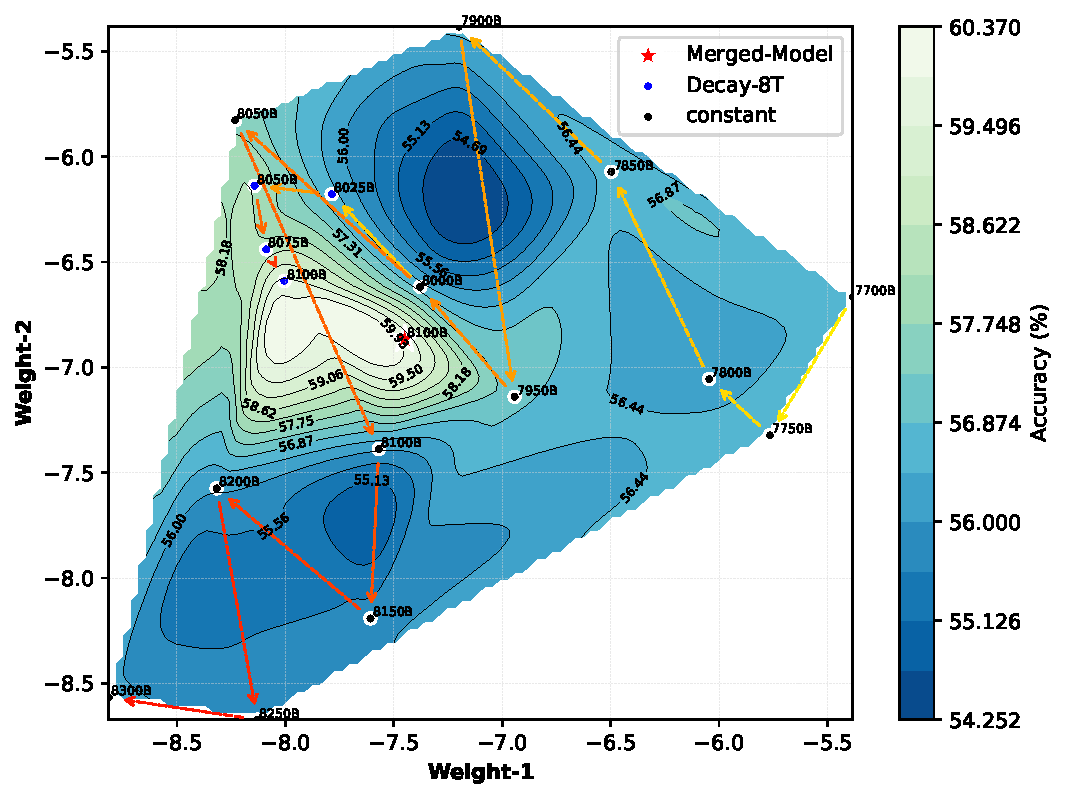
\includegraphics[width=0.8\textwidth]{figs/wss_ling_mini_merge_ckpt_weight_distributions_for_paper.pdf}
    \caption{\textbf{Visualization of Model Parameters and Performance Contour Lines.} Points connected by directional arrows represent parameter trajectories during the constant and decay phases, respectively. The red star indicates the solution space of the merged model.}
    \label{fig:wss_ling_mini_merge_ckpt_weight_distributions_for_paper}
\end{figure*}
